\documentclass[11pt, a4paper]{article}
\usepackage{setspace}
\usepackage[utf8]{inputenc}
\usepackage[mathlines]{lineno}
\usepackage{parskip}
\usepackage{graphicx}
\usepackage[margin=2cm]{geometry}
\usepackage{float}
\usepackage[scaled]{helvet}
\renewcommand\familydefault{\sfdefault} 
\usepackage[T1]{fontenc}
\graphicspath{ {./} }

\onehalfspacing
\begin{document}
\begin{titlepage}
    \begin{center}
        \vspace*{1cm}
            
        \Huge
        \textbf{Logistic model best fits population growth data using ordinary Linear and Non-linear model fitting methods}
        
        \vspace{2cm}
            
        \textbf{Junyue Zhang}
            
        \vfill
            
        This report is presented for the Computing Miniproject
        
        \vspace{0.8cm}
            
        \Large
        \textbf{Life Sciences}\\
        \textbf{Imperial College London}\\
        \textbf{03 December 2021}\\
        \textbf{Word count: 3480} 
            
    \end{center}
\end{titlepage}
\runninglinenumbers

\section{Six keywords}
Ocean, carbon sink, temperature, sinking rate, consumption rate, transfer efficiency

\section{Project ideas and proposed questions}
The concentration of carbon dioxide (CO2) in the atmosphere is strongly affected by the generation, sinking, and subsequent remineralization of the particulate organic carbon (POC) in the ocean (Marsay et al., 2015). The biological carbon sink in the ocean is propelled by plankton. They absorb carbon dioxide from the atmosphere and transform it into organic matter. After that, some dead plankton or their faeces sink from the upper ocean to the deep ocean (Guidi et al., 2016). However, the particulate organic carbon is consumed by some organisms such as zooplankton and bacteria during the sinking process (Buesseler and Boyd, 2009). Only no more than 10\% of the plankton carbon exported from the ocean surface is effectively deposited and sequestered in the deep layer on climatologically relevant timescales (Legendre et al., 2015).

Numerous studies have endeavored to investigate the particulate organic carbon (POC) sinking rates and consumption rates. Both these two rates are temperature dependent and can be used to describe the attenuation of sinking POC fluxes (Cavan et al., 2017). However, previous studies often oversimplify this important parameterization. Therefore, the research questions are as follows:

A. What is the particle sinking rate?

B. What is the consumption rate?

C. What is the transfer efficiency of the POC?

D. What controls the attenuation (or transfer efficiency) of the sinking carbon with the depth of the ocean?
  
\section{Proposed methods}
This project will use an already published data set of global particulate organic carbon fluxes (Mouw et al., 2015) to fit an exponential equation (equation 1) which is shown below.
\begin{equation}
F_z = F_{z0}e^{-(z-z_0)/z^*}
\end{equation}
This exponential equation links POC flux at any depth to flux measured at a reference depth by the remineralisation length scale z\textsuperscript{*} (Marsay et al., 2015). The equation used to calculate z\textsuperscript{*} is as follows (equation 2):
\begin{equation}
z^* = w / k
\end{equation}
where k is the remineralised turnover rate (d\textsuperscript{-1}) and w is the sinking rate (md\textsuperscript{-1}). z\textsuperscript{*} represents the depth (m) at which 63\% of the POC flux had been remineralised (Cavan et al., 2017). In addition, this project is a coding desk-based analysis. Python or R will be adopted to handle large spatial data sets, fit the model, and plot some graphs.

\section{Anticipated outputs and outcomes}
The anticipated outcomes are to accurately determine the POC sinking rates and turnover rates (remineralised) as well as the transfer efficiency of the sinking carbon. Furthermore, it is anticipated to use ecological theory to connect temperature with organism metabolic rates to determine the factors controlling the attenuation of POC flux with the ocean depth. This project will contribute toward a body of work to better parameterise Earth System Models used in climate projections.

\section{Project feasibility}
This project mainly includes literature review, data wrangling, model analysis, model fitting, data visualization, results analysis, writing report draft, report modification, and preparing for presentation \& viva. Since the data set has already been published and there are five months available for this project, so the project is considered feasible and achievable. A Gantt chart is shown below (figure 1).
\begin{figure}[H]
    \centering
    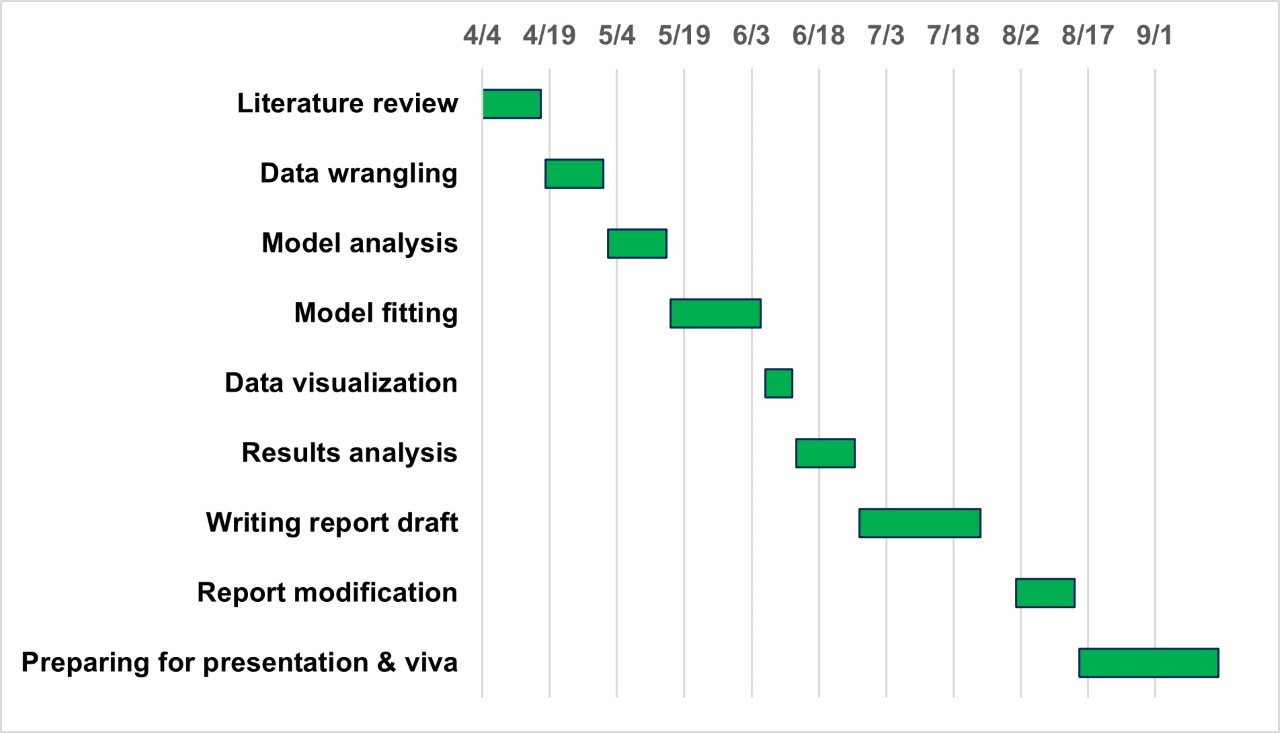
\includegraphics[width=0.8\textwidth]{gantt.jpg}
    \caption{Project Gantt chart}
    \label{figure1}
\end{figure}
\section{An itemized budget}
This project is free.
\section{Cited references}
 Buesseler, K. O., \& Boyd, P. W. (2009). Shedding light on processes that control particle export and flux attenuation in the twilight zone of the open ocean. Limnology and Oceanography, 54(4), 1210-1232.

Cavan, E. L., Trimmer, M., Shelley, F., \& Sanders, R. (2017). Remineralization of particulate organic carbon in an ocean oxygen minimum zone. Nature Communications, 8(1), 1-9.

Guidi, L., Chaffron, S., Bittner, L., Eveillard, D., Larhlimi, A., Roux, S., ... \& Gorsky, G. (2016). Plankton networks driving carbon export in the oligotrophic ocean. Nature, 532(7600), 465-470.

Legendre, L., Rivkin, R. B., Weinbauer, M. G., Guidi, L., \& Uitz, J. (2015). The microbial carbon pump concept: Potential biogeochemical significance in the globally changing ocean. Progress in Oceanography, 134, 432-450.

Marsay, C. M., Sanders, R. J., Henson, S. A., Pabortsava, K., Achterberg, E. P., \& Lampitt, R. S. (2015). Attenuation of sinking particulate organic carbon flux through the mesopelagic ocean. Proceedings of the National Academy of Sciences, 112(4), 1089-1094.
\end{document}

